We start with a post out in the Fediverse that sets a scene. Quoting
@rbreich@masto.ai: \url{https://masto.ai/@rbreich/110211057046354723}
\#retoot

\begin{figure}
\centering
\pandocbounded{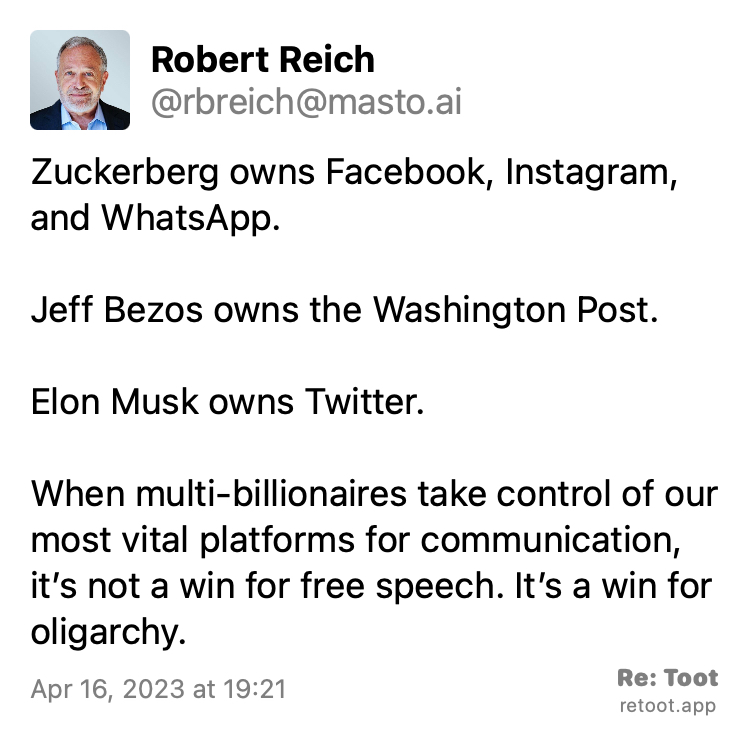
\includegraphics[keepaspectratio]{\%7B\%7Bsite.url\%7D\%7D/img/rbreich-oligarchs.jpg}}
\caption{Post by Robert Reich. ``Zuckerberg owns Facebook, Instagram,
and WhatsApp. Jeff Bezos owns the Washington Post. Elon Musk owns
Twitter. When multi-billionaires take control of our most vital
platforms for communication, it's not a win for free speech. It's a win
for oligarchy.'' Posted on Apr 16, 2023 at 19:21}
\end{figure}

What can we do about this? I wish I had solutions. AM radio stations are
still closing left and right across the country. Harry McCracken
recently wrote about
\href{https://web.archive.org/web/20230416142822/https://www.technologizer.com/2023/04/15/the-end-of-computer-magazines-in-america/}{an
entire genre of print publications disappearing}. Our economy is far
more fragile than it seems at first glance.

Yeah, I'm getting that Weimar sort of feeling.
